\documentclass[11pt, a4paper]{article}		% general format


%%%% Charset
\usepackage[utf8]{inputenc}					% use utf8					
\usepackage[russian]{babel}					% use russian font


%%%% Math
\usepackage{amsmath}						% Amer­i­can Math­e­mat­i­cal So­ci­ety (AMS) math fa­cil­i­ties
\usepackage{amsfonts}						% fonts from the AMS
\usepackage{amssymb}						% additional math symbols


%%%% Graphics
\usepackage{graphicx}


\author{Дедков Сергей}
\title{An Empirical Study of Cryptographic Misuse in Android Applications}
\date{2015}

%---------------------------------------------------------

\begin{document}
\maketitle
%---------------------------------------------------------

\section{An Empirical Study of Cryptographic Misuse in Android Applications}

Авторы данной статьи опросили разработчиков, используют ли они криптографические API, которые обеспечивают криптографическую безопасность.
Разработали методы анализа и проанализировали Google Play рынок, обнаружив, что 10327 из 11748 приложений - используют криптографические интерфейсы. 88\% допустили хотя бы одну ошибку.

Разработчики используют криптографические примитивы, такие как блочные шифры и код аутентфикации сообщения(MAC) для защиты данных и связи. Криптографы знают, что есть правильный способ и неправильный способ использовать эти примитивы, где правильный способ обеспечивает надежные гарантии безопасности, а неправильный способ неизменно приводит к уязвимостям.

Сосредоточились авторы на двух стандартах безопасности: атаки по выбранным открытым текстам (IND-CPA) и стойкости к уязвимостям.

При этом платформа Android была выбрана не случайно, для этого были следующие причины:

\begin{itemize}

\item Приложения запускаются на мобильных платформах, которые хранят множество персональной информации

\item Приложения пишкться на Java. А Java’s cryptographic API достаточно стабильна.

\item Под Android написано очень много приложений, на основе которых формировалась база статисктики, в которой были отражены способы использования криптографических примитивов пользователями.

\end{itemize}

Для выявления дефектов был использован статический анализатор уязвимостей CryptoLint, основанный на Androguard Android. Результаты были приведены выше.

Авторы предлжили 6 правил. Любое приложение, которое нарушает одно из них не может быть безопасным:

\begin{itemize}

\item[-] Не используйте режим ECB для шифрования. 

\begin{figure}[h!]
	\centering
	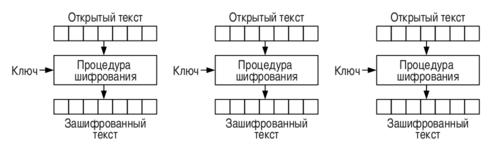
\includegraphics[scale=0.80]{res/ecb_mode}
	\caption{Шифрование в режиме ECB (режиме электронной кодовой книги)}
\end{figure}

Используя режим ECB, разарботчики подвергают свое ПО уязвимостям. Такой режим уязвим, т.к. в нем одинаковые фрагменты шифруются в одинаковую последовательность(см. рисунок 1). Для предотвращения к блокам добавляют соль, для более сложного взлома.

\item[-] Не используйте неслучайный IV (вектор инициализации см. рисунок 2) для шифрования CBC.

\begin{figure}[h!]
	\centering
	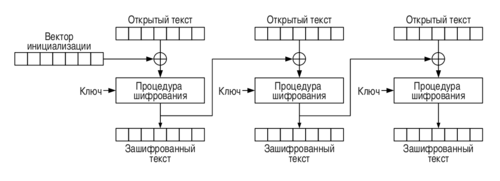
\includegraphics[scale=0.80]{res/cbc_mode}
	\caption{Шифрование в режиме CBC (режиме сцепления блоков шифротекста)}
\end{figure}

Использование неслучайного вектора инициализации повышает криптостойкость системы.

\item[-] Не использовать постоянные ключи шифрования.

Смысл такой же, как и у второго правила.

\item[-] Не используйте постоянные соли для РВЕ.

Статическая соль и тому подобные конструкции могут служить достаточно хорошо, пока структура этих конструкций и соль хранятся в тайне. Если же злоумышленник вызнает секрет хэширования — он с легкостью сможет использовать в своих целях.

\item[-] Не используйте меньше 1000 итераций для РВЕ.

\item[-]  Не использовать постоянные seed для получения псевдослучайных последовательностей SecureRandom.

Правило 4 и 5 выведено чисто опытным путем для PBE схем.

\end{itemize}

CrytpoLint после анализа указывает соблюда.тся ли эти 6 правил.

В отличие от обычных java-приложений Android-приложение запускается на виртуальной машине Dalvik. С этим байкодом и работает инструмент авторов - CryptoLint. Приложения, которые запускаются на виртуальной машине Dalvik получают доступ к интерфейсу и подсистемам. Для получения доступа к алгоритмам шифрования вызывается метод Cipher.getInstance, которые зарегистрированы в cryptographic service providers
(CSP), в подсистеме Java Cryptography Architecture (JCA). 

В такой реализации по-умолчанию выбирается ECB шифрование. Авторами проводились исселдования графа потока управления приложения и то, как находились нарушения. В качестве примера было рассмотрено 3 популярных приложения с уязвимостями, при этом эти приложения имели миллионы скачиваний. 

\end{document}